%% ================================================================
%% Security Vulnerabilities in Modern IP Surveillance Networks:
%% A Systematic Review of Edge-Device Attacks
%%
%% Author: Maheen Fatima
%% IEEE Conference Format (ieeeconf.cls)
%%
%% FINAL VERSION WITH TIKZ FIGURES — April 2026
%%   Figure 1: Four-Tier Attack Surface Architecture Diagram
%%             (placed at end of Section II – Literature Review)
%%   Figure 2: Firmware Analysis & Vulnerability Discovery Flowchart
%%             (placed at end of Section III – Methodology)
%% ================================================================

\documentclass[letterpaper, 10pt, conference]{ieeeconf}
\IEEEoverridecommandlockouts
\overrideIEEEmargins

%% ----------------------------------------------------------------
%% Standard packages
%% ----------------------------------------------------------------
\usepackage[utf8]{inputenc}
\usepackage[T1]{fontenc}
\usepackage{cite}
\usepackage{amsmath}
\usepackage{amssymb}
\usepackage{graphicx}
\usepackage{booktabs}
\usepackage{array}
\usepackage{url}
\usepackage[hidelinks]{hyperref}
\hypersetup{
  colorlinks=true,
  linkcolor=blue,
  citecolor=blue,
  urlcolor=blue
}
\usepackage{multirow}
\usepackage{tabularx}
\usepackage{rotating}
\usepackage{makecell}
\usepackage{balance}  % column balancing for bibliography

%% ----------------------------------------------------------------
%% TikZ packages required for both figures
%% ----------------------------------------------------------------
\usepackage{tikz}
\usetikzlibrary{
  shapes.geometric,   % diamond decision nodes
  shapes.symbols,     % document shape
  shapes.misc,        % rounded rectangles
  arrows,             % legacy arrow tips (required for copy shadow)
  arrows.meta,        % modern arrow tips
  positioning,        % relative node placement (right of, below of, etc.)
  fit,                % bounding-box nodes around groups
  backgrounds,        % layered drawing for shaded regions
  calc,               % coordinate arithmetic
  shadows,            % copy shadow for flowchart blocks
  shadows.blur        % subtle drop shadows on hardware block
}
\usepackage{pgfplots}
\pgfplotsset{compat=1.18}

%% ----------------------------------------------------------------
%% Convenience colour definitions (IEEE-friendly, no garish colours)
%% ----------------------------------------------------------------
\definecolor{layerI}{RGB}{180,30,30}      % Physical  – dark red
\definecolor{layerII}{RGB}{20,80,160}     % Protocol  – IEEE blue
\definecolor{layerIII}{RGB}{30,120,50}    % Firmware  – dark green
\definecolor{layerIV}{RGB}{130,50,160}    % Perception – purple
\definecolor{hwfill}{RGB}{230,230,240}    % hardware block fill
\definecolor{netfill}{RGB}{220,235,255}   % network zone fill
\definecolor{cloudfill}{RGB}{240,248,220} % cloud zone fill
\definecolor{envfill}{RGB}{255,245,220}   % environment zone fill
\definecolor{boxgray}{RGB}{245,245,245}   % generic light box
\definecolor{decisionfill}{RGB}{255,250,210} % decision diamond fill

%% ----------------------------------------------------------------
%% Title and author
%% ----------------------------------------------------------------
\title{\LARGE \bf
Security Vulnerabilities in Modern IP Surveillance Networks:
A Systematic Review of Edge-Device Attacks
}

\author{Maheen Fatima$^{1}$%
\thanks{$^{1}$Maheen Fatima is with the Department of Information
Technology, PUCIT, Lahore, Pakistan.
{\tt\small bitf22m031@pucit.edu.pk}}%
}

\begin{document}

\maketitle
\thispagestyle{empty}
\pagestyle{empty}

%% ================================================================
\begin{abstract}

The contemporary Internet Protocol (IP) surveillance camera has undergone
a fundamental architectural transformation, evolving from a passive,
analog-adjacent recording appliance into a fully networked Linux-based
edge computing node capable of autonomous inference, bidirectional cloud
synchronization, and multi-protocol service hosting. This architectural
evolution has produced an attack surface of unprecedented breadth and
depth, spanning physical hardware interfaces, embedded firmware
binaries, application-layer network protocols, and the logic of embedded
perception pipelines. This paper presents a systematic, multi-tier
vulnerability taxonomy for modern IP surveillance infrastructure, organized
across four distinct threat layers: (I) Physical and Hardware, encompassing
UART/JTAG interface abuse and flash chip extraction; (II) Protocol-Layer,
addressing structural weaknesses in the Real-Time Streaming Protocol (RTSP,
RFC 2326), the ONVIF device management framework, and associated
authentication mechanisms; (III) Firmware and Application-Layer, covering
static and dynamic binary exploitation, memory-corruption vulnerabilities,
web-interface Cross-Site Request Forgery (CSRF), and supply-chain SDK
weaknesses; and (IV) Perception-Layer Protocol Vulnerabilities, a novel
framing of adversarial inputs as logic-level protocol exploits against the
inference services exposed by smart edge cameras. Drawing on 15 verified,
peer-reviewed sources including the landmark Sensors 2020 survey by Kalbo
et al., the IWSEC 2024 Tenda CP3 firmware study by Stabili et al., and
confirmed Common Vulnerabilities and Exposures (CVE) records with CVSS
scores reaching 9.8 (Critical), this paper constructs a detailed
comparative threat matrix, presents a structured vulnerability discovery
methodology grounded in Binwalk, Ghidra, and context-aware binary triage
via the rhabdomancer plugin, and proposes a cross-layer mitigation
framework incorporating Zero Trust Architecture (ZTA) aligned with NIST
SP~800-207, Secure RTSP (RTSPS), and hardware-level Root-of-Trust (RoT).
Our analysis demonstrates that effective defense of IP surveillance
infrastructure is not achievable through any single control layer and
requires the coordinated application of hardware, protocol, and
system-level security primitives.

\end{abstract}

%% ================================================================
\section{INTRODUCTION}

The global market for Internet Protocol video surveillance was valued at
approximately \$53.7~billion in 2023 and is projected to reach
\$83.3~billion by 2028, driven predominantly by the replacement of analog
CCTV infrastructure with network-addressable smart devices \cite{kalbo2020}.
This transition carries security implications of a qualitatively different
order than those associated with legacy surveillance systems. Where an
analog CCTV camera's attack surface was bounded by physical wire cutting
and local recording-unit tampering \cite{kalbo2020}, a modern IP camera
is a fully provisioned Linux computer, hosting a web management server,
an RTSP streaming daemon, an ONVIF device discovery interface,
a cloud synchronization agent, and---in an increasing proportion of
deployed units---an on-device inference engine executing deep neural
network models for object detection, facial recognition, and behavioral
analytics \cite{jin2022edge}. Each of these services constitutes an
independently exploitable attack surface, and the convergence of these
surfaces on a single edge device transforms a passive monitoring
appliance into a high-value network intrusion target.

The kinetic consequences of inadequately secured surveillance
infrastructure were concretely demonstrated in January 2024, when
Ukrainian security services confirmed that an Internet Protocol camera
positioned to monitor a residential parking facility in an area
subject to conflict had been compromised and co-opted by adversaries
to conduct pre-strike reconnaissance prior to a missile attack
\cite{asimily2024}. This incident represents a categorical escalation
in the operational significance of IP camera security, from a matter
of privacy and data confidentiality to one of physical safety and
national security. It establishes definitively that the security
posture of surveillance edge devices is not a marginal technical
concern but a matter of critical infrastructure protection.

At the network layer, the scale of exposure is staggering. Kalbo et al.
conducted systematic enumeration of Internet-facing surveillance
infrastructure using the Shodan and Censys search engines and identified
over one million IP cameras and more than 125,000 surveillance recording
servers directly accessible on the public Internet, with approximately
90\% of these devices communicating management interfaces over unencrypted
HTTP rather than HTTPS \cite{kalbo2020}. A complementary 2024 study by
Ng and Mehrnezhad examining 281 UK-registered cameras indexed on Shodan
found that a majority exposed unauthenticated Real-Time Streaming Protocol
(RTSP) video feeds, with over 76\% installed in residential environments
\cite{ng2024shodan}. These statistics establish not merely the existence
of vulnerabilities but their systematic, large-scale deployment at
global scope.

At the firmware layer, the 2024 study by Stabili et al.~\cite{stabili2024},
published at the IWSEC 2024 workshop in Kyoto and indexed in Springer
Lecture Notes in Computer Science, represents the most methodologically
complete public analysis of a consumer IP camera as of the time of
writing. The authors applied hardware extraction, static binary analysis
via Ghidra augmented by the context-aware rhabdomancer plugin, and
dynamic validation to the Tenda CP3 consumer camera, yielding five
novel CVEs with Common Vulnerability Scoring System (CVSS) scores
ranging from 7.5 to 9.8~\cite{stabili2024}. That a coordinated
disclosure process initiated in June 2023 had resulted in no manufacturer
response or patch release by the time of publication in September 2024
illustrates the systemic inadequacy of vulnerability lifecycle management
in the consumer surveillance hardware industry.

The final tier of the threat landscape, and the one most critically
underexamined in the cybersecurity literature, concerns what this paper
terms \textit{Perception-Layer Protocol Vulnerabilities}: exploits that
target the inference logic of embedded smart camera systems through
structurally crafted physical inputs, analogous to a malformed network
packet that exploits a parsing flaw, but operating at the optical and
physical input layer. Sharif et al.'s foundational ACM CCS 2016
work on adversarial biometric bypass \cite{sharif2016}, and Thys
et al.'s demonstration of adversarial logic-bypass of automated perimeter
monitoring \cite{thys2019}, are appropriately framed within this
taxonomy as protocol-level exploits against the inference service layer
of smart edge cameras, rather than as machine learning curiosities.

This paper makes the following contributions: (1) a four-tier IP
surveillance threat taxonomy anchored to real CVE disclosures and
verified academic sources; (2) a detailed, reproducible vulnerability
discovery methodology covering hardware extraction through binary
fuzzing; (3) a quantitative comparative analysis table of threat
vectors by exploitability, cost, and CVSS severity; (4) case-study
integration of the Tenda CP3 firmware analysis and the Sharif et al.
biometric bypass; and (5) a cross-layer mitigation framework grounded
in NIST SP~800-207 Zero Trust Architecture, RTSPS, and hardware RoT.

%% ================================================================
\section{LITERATURE REVIEW}

The academic treatment of IP surveillance security has evolved
significantly over the decade since the Mirai botnet incident of
August--October 2016, which assembled a corpus exceeding 600,000
compromised IoT devices---predominantly IP cameras and digital video
recorders operating with factory-default credentials---into a
distributed denial-of-service platform capable of sustaining attack
traffic in excess of 1~Tbps \cite{kambourakis2017}. Kambourakis et al.
provide the definitive academic characterization of this event,
identifying the structural enabler as the combination of default
credential persistence and unrestricted Telnet service exposure across
millions of devices whose manufacturers had made no provision for
security testing or coordinated vulnerability response \cite{kambourakis2017}.
The Mirai incident established the empirical foundation for a research
agenda that has since expanded to address the full depth of the
IP surveillance threat landscape.

The seminal architectural survey by Kalbo et al.~\cite{kalbo2020}
represents the most comprehensive single treatment of the IP video
surveillance attack surface in the literature. The authors decompose
the system into five layers---camera hardware, network infrastructure,
video management server, client applications, and cloud backend---and
analyze the attack surface at each layer. Their Shodan enumeration
methodology, which identified over one million Internet-facing cameras,
provides the quantitative grounding for understanding the real-world
scope of the problem. The survey additionally introduces the video
injection attack class, in which an adversary who has intercepted
an unencrypted RTSP stream between a camera and its recording server
substitutes a pre-recorded or synthetically generated feed, causing
security personnel to operate on falsified situational awareness data.
This attack class, enabled by the absence of transport-layer
encryption on RTSP streams documented by Santos et al.~\cite{santos2023},
represents a particularly severe operational threat in high-stakes
surveillance environments.

The structural analysis of RTSP protocol vulnerabilities by Santos et
al.~\cite{santos2023} establishes four weakness classes inherent to
common RTSP implementations: unencrypted streaming server URL disclosure;
cleartext transmission of user, Wi-Fi, and RTSP credentials; absent
input validation for RTSP request parameters (CWE-20); and missing
replay-attack protection. These weaknesses are substantially attributable
to the RTSP specification itself, which predates modern security
engineering norms and does not mandate authentication by default
\cite{santos2023}. The ONVIF specification, which governs device
discovery and profile management in enterprise-grade IP camera
deployments, introduces additional exposure: CVE-2022-30563 documented
an attack against Dahua's IP cameras in which an adversary could
intercept unencrypted ONVIF session traffic and replay the user's
login packet to obtain full administrative access \cite{securithings2022}.

At the embedded systems layer, the foundational survey by Charmanas
et al.~\cite{charmanas2023} characterizes the complete pipeline of IoT
firmware security analysis, from hardware-based extraction via UART
and JTAG through static analysis frameworks to dynamic emulation
environments. The review by Feng et al.~\cite{feng2023}, published
in the IEEE/CAA Journal of Automatica Sinica, surveys firmware
vulnerability detection techniques applicable to IoT binaries with
particular attention to taint analysis, symbolic execution, and
coverage-guided fuzzing in emulated environments. The Firmadyne-based
analysis framework described by Andriesse et al. and further developed
in the FirmAE extended emulation system \cite{firmae2020} establishes
the practical foundation for automated dynamic testing of Linux-based
camera firmware, enabling systematic fuzzing of the CGI and web
management interfaces that represent the most commonly exploited
remote attack surface.

In the domain of edge security architecture, Jin et al.~\cite{jin2022edge}
provide a systematic treatment of security threats emerging from edge
computing paradigms, specifically documenting how the hardware-to-system
vulnerability stack manifests in edge deployments and arguing for a
holistic cross-layer analysis posture. The risk quantification work
of Bhardwaj et al.~\cite{bhardwaj2024}, which applies Bayesian hazard
graphs and CVSS-integrated conditional probability tables to IoT camera
risk scoring, provides the methodological foundation for dynamic,
continuous risk assessment at the camera fleet level. Yeboah-Ofori
et al.~\cite{yeboah2023} characterize the Evil Twin Man-in-the-Middle
attack in smart camera networks, providing a kill-chain model for
this attack class and demonstrating empirically that absent certificate
pinning in camera mobile applications and insufficient Wi-Fi security
protocols are the primary enablers of successful interception.

Figure~\ref{fig:attack_surface} synthesizes the four-tier taxonomy
across the complete IP surveillance system architecture described in
this review.

%% ================================================================
%% FIGURE 1 — Four-Tier Attack Surface Architecture Diagram
%% Placed immediately after the Literature Review summary paragraph.
%% Uses tikz: shapes.geometric, positioning, fit, backgrounds, calc
%% ================================================================

\begin{figure*}[t]
\centering
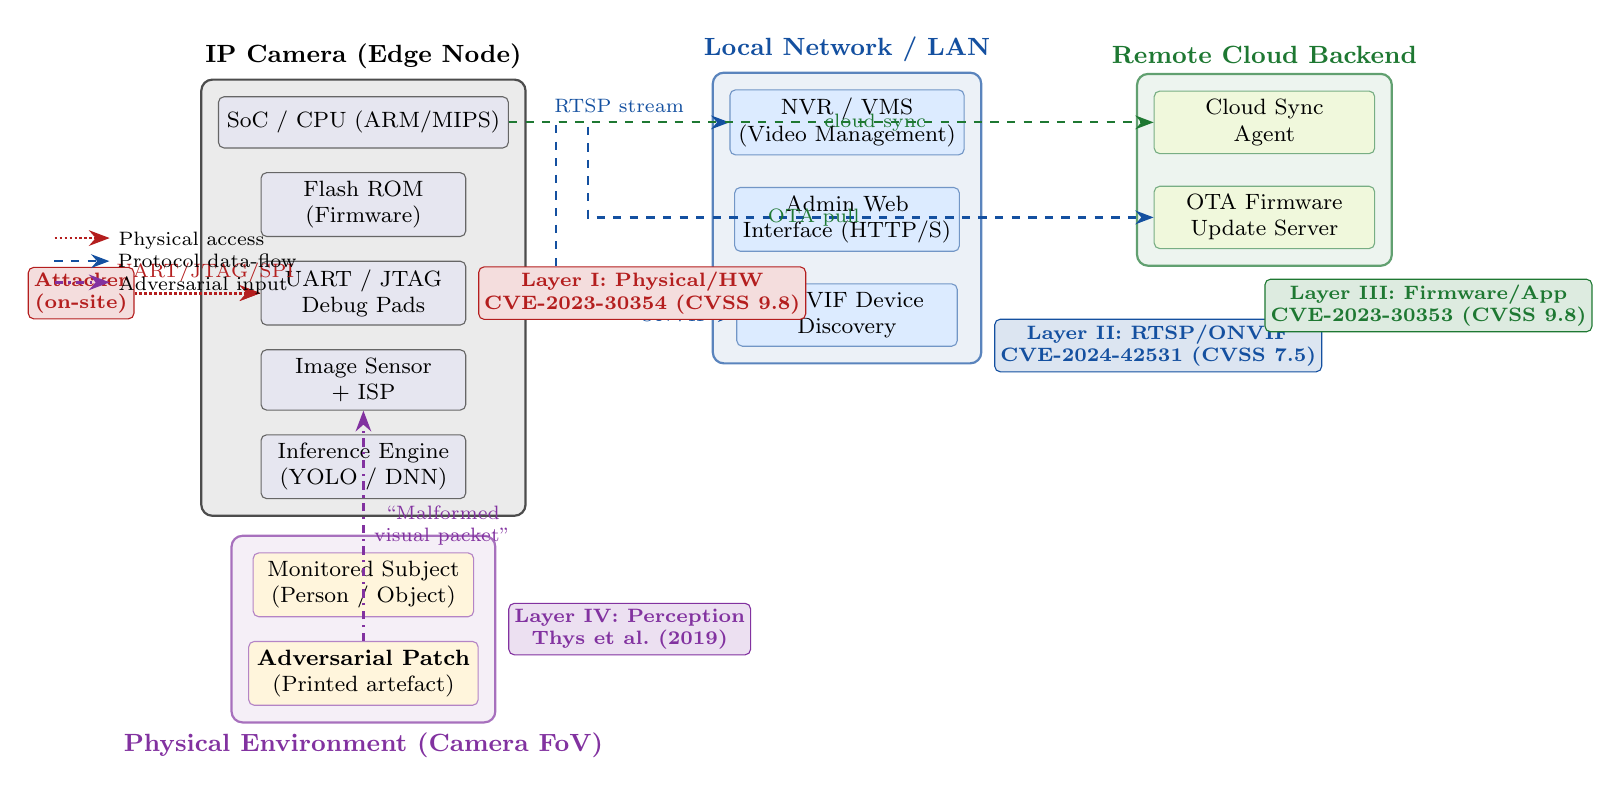
\begin{tikzpicture}[
  %% --- global style definitions ---
  >=Stealth,
  font=\footnotesize,
  %% hardware sub-block style
  hwblock/.style={
    rectangle, rounded corners=2pt,
    draw=black!60, fill=hwfill,
    minimum width=2.6cm, minimum height=0.55cm,
    align=center, inner sep=3pt
  },
  %% external zone box style
  zonebox/.style={
    rectangle, rounded corners=4pt,
    draw=#1!70, fill=#1!8,
    inner sep=6pt, line width=0.8pt
  },
  %% threat-layer annotation pill
  threatpill/.style={
    rectangle, rounded corners=2pt,
    draw=#1, fill=#1!15,
    font=\scriptsize\bfseries,
    inner sep=2pt, text=#1
  },
  %% network data-flow arrow
  dataflow/.style={
    ->, draw=layerII, thick, dashed
  },
  %% physical-threat arrow
  physarrow/.style={
    ->, draw=layerI, thick, densely dotted, line width=1pt
  },
  %% adversarial input arrow
  advarrow/.style={
    ->, draw=layerIV, thick, dash dot, line width=1pt
  }
]

%% ============================================================
%% ZONE A — IP Camera Hardware (centre-left)
%% ============================================================
\node[hwblock, minimum width=2.8cm, minimum height=0.65cm]
  (soc)  at (0,0)   {SoC / CPU (ARM/MIPS)};
\node[hwblock, below=0.30cm of soc]
  (flash){Flash ROM\\(Firmware)};
\node[hwblock, below=0.30cm of flash]
  (uart) {UART / JTAG\\Debug Pads};
\node[hwblock, below=0.30cm of uart]
  (lens) {Image Sensor\\+ ISP};
\node[hwblock, below=0.30cm of lens]
  (nn)   {Inference Engine\\(YOLO / DNN)};

%% Bounding box around the camera hardware
\begin{scope}[on background layer]
  \node[zonebox=black, fit=(soc)(flash)(uart)(lens)(nn),
        label={[font=\small\bfseries]above:IP Camera (Edge Node)}]
        (cambox) {};
\end{scope}

%% ============================================================
%% ZONE B — Local Network / NVR  (right of camera)
%% ============================================================
\node[hwblock, minimum width=2.8cm, right=2.8cm of soc,
      fill=netfill, draw=layerII!60]
  (nvr)  {NVR / VMS\\(Video Management)};
\node[hwblock, minimum width=2.8cm, below=0.40cm of nvr,
      fill=netfill, draw=layerII!60]
  (mgmt) {Admin Web\\Interface (HTTP/S)};
\node[hwblock, minimum width=2.8cm, below=0.40cm of mgmt,
      fill=netfill, draw=layerII!60]
  (onvif){ONVIF Device\\Discovery};

\begin{scope}[on background layer]
  \node[zonebox=layerII, fit=(nvr)(mgmt)(onvif),
        label={[font=\small\bfseries, text=layerII]above:Local Network / LAN}]
        (netbox) {};
\end{scope}

%% ============================================================
%% ZONE C — Cloud Backend  (far right)
%% ============================================================
\node[hwblock, minimum width=2.8cm, right=2.4cm of nvr,
      fill=cloudfill, draw=layerIII!60]
  (cloud){Cloud Sync\\Agent};
\node[hwblock, minimum width=2.8cm, below=0.40cm of cloud,
      fill=cloudfill, draw=layerIII!60]
  (ota)  {OTA Firmware\\Update Server};

\begin{scope}[on background layer]
  \node[zonebox=layerIII, fit=(cloud)(ota),
        label={[font=\small\bfseries, text=layerIII]above:Remote Cloud Backend}]
        (cloudbox) {};
\end{scope}

%% ============================================================
%% ZONE D — Physical Environment (below camera)
%% ============================================================
\node[hwblock, minimum width=2.8cm, below=1.8cm of lens,
      fill=envfill, draw=layerIV!60]
  (person){Monitored Subject\\(Person / Object)};
\node[hwblock, minimum width=2.8cm, below=0.30cm of person,
      fill=envfill, draw=layerIV!60]
  (patch) {\textbf{Adversarial Patch}\\(Printed artefact)};

\begin{scope}[on background layer]
  \node[zonebox=layerIV, fit=(person)(patch),
        label={[font=\small\bfseries, text=layerIV]below:Physical Environment (Camera FoV)}]
        (envbox) {};
\end{scope}

%% ============================================================
%% DATA-FLOW ARROWS (dashed blue — Layer II protocol streams)
%% ============================================================
\draw[dataflow]
  (soc.east) -- node[above, font=\scriptsize, text=layerII]
  {RTSP stream} (nvr.west);

\draw[dataflow]
  (soc.east) -- ++(0.6,0) |- node[right, font=\scriptsize,
  text=layerII, pos=0.7] {ONVIF} (onvif.west);

\draw[dataflow]
  (soc.east) -- ++(1.0,0) |- node[right, font=\scriptsize,
  text=layerIII, pos=0.65] {OTA pull} (ota.west);

\draw[dataflow, draw=layerIII]
  (soc.east) -- ++(1.0,0) |- node[right, font=\scriptsize,
  text=layerIII, pos=0.7] {cloud sync} (cloud.west);

%% ============================================================
%% PHYSICAL-ACCESS ARROW (dotted red — Layer I)
%% ============================================================
\draw[physarrow]
  ([xshift=-1.4cm]uart.west) --
  node[above, sloped, font=\scriptsize, text=layerI]
  {UART/JTAG/SPI} (uart.west);

%% Label the physical attacker
\node[threatpill=layerI, left=1.6cm of uart, align=center]
  (attI) {Attacker\\(on-site)};

\draw[physarrow] (attI.east) -- (uart.west);

%% ============================================================
%% ADVERSARIAL-INPUT ARROW (dash-dot purple — Layer IV)
%% ============================================================
\draw[advarrow]
  (patch.north) -- node[right, font=\scriptsize, text=layerIV]
  {\shortstack{``Malformed\\visual packet''}} (lens.south);

%% ============================================================
%% THREAT-LAYER ANNOTATION PILLS — placed alongside each zone
%% ============================================================

%% Layer I label (Physical) — annotates UART block
\node[threatpill=layerI, right=0.15cm of uart, align=center,
      font=\scriptsize\bfseries]
  {\textbf{Layer I:} Physical/HW\\CVE-2023-30354 (CVSS~9.8)};

%% Layer II label (Protocol) — annotates NVR zone
\node[threatpill=layerII, above right=-0.1cm and 0.15cm of netbox.south east,
      align=center, font=\scriptsize\bfseries]
  {\textbf{Layer II:} RTSP/ONVIF\\CVE-2024-42531 (CVSS~7.5)};

%% Layer III label (Firmware) — annotates cloud zone
\node[threatpill=layerIII, below right=0.15cm and 0.0cm of cloudbox.south,
      align=center, font=\scriptsize\bfseries]
  {\textbf{Layer III:} Firmware/App\\CVE-2023-30353 (CVSS~9.8)};

%% Layer IV label (Perception) — annotates env zone
\node[threatpill=layerIV, right=0.15cm of envbox.east,
      align=center, font=\scriptsize\bfseries]
  {\textbf{Layer IV:} Perception\\Thys et al.\ (2019)};

%% ============================================================
%% LEGEND (bottom-left)
%% ============================================================
\node[align=left, font=\scriptsize, anchor=south west]
  at ([xshift=0.2cm, yshift=0.2cm]attI.south west)
  {%
    \tikz\draw[physarrow,>=Stealth] (0,0)--(0.7,0); Physical access\\
    \tikz\draw[dataflow,>=Stealth] (0,0)--(0.7,0); Protocol data-flow\\
    \tikz\draw[advarrow,>=Stealth] (0,0)--(0.7,0); Adversarial input%
  };

\end{tikzpicture}

\caption{Four-Tier IP Surveillance Attack Surface. The IP camera
edge node (centre) is simultaneously exposed to: \textbf{Layer~I}
physical attacks via debug interfaces (UART/JTAG); \textbf{Layer~II}
protocol attacks over RTSP and ONVIF streams to the local NVR;
\textbf{Layer~III} firmware and supply-chain attacks through the
cloud OTA update channel; and \textbf{Layer~IV} perception-layer
attacks in which a physically realized adversarial patch injects a
semantically malformed visual input into the camera's inference
pipeline~\cite{thys2019,sharif2016}.}
\label{fig:attack_surface}
\end{figure*}

%% ================================================================
\section{VULNERABILITY DISCOVERY METHODOLOGY}

The discovery of exploitable vulnerabilities in IP surveillance edge
devices requires a multi-stage analytical pipeline that addresses
both the hardware substrate and the firmware it executes. This section
describes the established methodology in the detail necessary for
reproducibility, as applied in the Tenda CP3 case study and
generalizable to the broad class of Linux-based IP cameras.
Figure~\ref{fig:flowchart} summarizes the complete pipeline.

\subsection{Phase 1: Open-Source Intelligence and Hardware Enumeration}

The initial phase applies Open-Source Intelligence (OSINT) techniques
to characterize the target device. The Federal Communications Commission
(FCC) ID database provides hardware photographs, internal layouts, and
sometimes regulatory test reports that identify the main processor
architecture, flash memory chip model, and the presence and location
of debug interface pads. Datasheet mining for the identified processor
and memory components establishes pin assignments for UART and JTAG
interfaces without requiring destructive analysis. Stabili et al.
\cite{stabili2024} employed this approach as the first phase of their
Tenda CP3 analysis, identifying the processor family and memory
topology prior to any physical intervention on the device.

\subsection{Phase 2: Hardware Extraction via UART and JTAG}

The Universal Asynchronous Receiver-Transmitter (UART) interface
is the most commonly accessible hardware debug surface on consumer
IP cameras \cite{charmanas2023}. UART pins can be identified by
probing exposed test points on the circuit board with a logic analyzer
or multimeter, and a compatible level-shifting adapter (typically
3.3~V) connects the device to a host terminal emulator. In the
majority of consumer-grade cameras, the UART interface provides
unrestricted access to the bootloader command shell: by interrupting
the boot sequence with a device-specific key combination during
power-on, an analyst can obtain a root shell on the running system
or redirect the boot to a recovery environment from which the full
filesystem can be archived \cite{charmanas2023, kaspersky2022}.
CVE-2023-30354 (CVSS 9.8), disclosed against the Tenda CP3, specifically
documents Wi-Fi credential leakage and unrestricted console access
achievable through this mechanism \cite{stabili2024}.

The JTAG (Joint Test Action Group) interface provides lower-level
capabilities: direct read and write access to device memory (both
ROM and RAM), hardware breakpoint insertion, and processor register
state inspection. When UART shells are locked by a boot password,
JTAG provides an alternative extraction path. Using an appropriate
JTAG programmer and the JTAGulator tool for automated pin
identification, an analyst can dump the complete flash memory
contents without decrypting or bypassing software-level access
controls \cite{charmanas2023}. For devices with neither accessible
UART nor JTAG---a rarer configuration in consumer hardware---direct
SPI or NAND flash chip reading via desoldering or test-clip connection
provides equivalent access to the raw firmware image.

\subsection{Phase 3: Static Firmware Analysis}

The raw firmware image, once acquired, is processed through the
Binwalk tool for signature-based detection and extraction of embedded
filesystems, compressed archives, kernel images, and cryptographic
material. Binwalk's entropy analysis identifies compressed or encrypted
regions whose boundaries delimit firmware subcomponents. Following
filesystem extraction, automated audit scripts such as Firmwalker
scan the extracted contents for high-value artifacts: password hash
files, private key material, hardcoded credentials in configuration
scripts, and CGI binary executables that process user-controlled input.

Binary analysis of extracted executables proceeds through the Ghidra
Software Reverse Engineering framework (developed and released by
the NSA), which provides decompilation of ARM and MIPS binaries---the
two dominant architectures in consumer IP cameras---into pseudo-C
representations amenable to manual audit. Stabili et al.~\cite{stabili2024}
augment the standard Ghidra workflow with the \textit{rhabdomancer}
plugin, which performs context-aware binary triage: rather than
applying generic vulnerability patterns uniformly across a large
firmware binary---an approach that produces unmanageable false-positive
volumes---rhabdomancer identifies functions that receive and process
data originating from network connections, constructing a call-graph
of network-data-reachable code paths. This focused triage directed
analyst attention to the specific code regions in which the five Tenda
CP3 CVEs were ultimately confirmed, demonstrating substantially improved
analytical efficiency over prior undifferentiated approaches.

\subsection{Phase 4: Dynamic Analysis and Fuzzing}

Dynamic analysis requires execution of firmware, either on the physical
device under a controlled network environment or within an emulated
system. The Firmadyne framework \cite{charmanas2023} provides automated
Linux firmware emulation under QEMU, modifying the Linux kernel to
handle peripheral exceptions arising from the absence of real hardware.
The FirmAE extension \cite{firmae2020} substantially improves emulation
fidelity, reportedly achieving successful emulation of 79.36\% of tested
firmware images. Within the emulated environment, the web management
interface and CGI handlers are accessible to network fuzzing tools.

Coverage-guided fuzzing---in which AFL (American Fuzzy Lop) or its
derivatives monitor code coverage to guide input mutation toward
unexplored execution paths---is applied to network-exposed service
interfaces to systematically identify memory-corruption vulnerabilities
including stack buffer overflows, heap overflows, and format-string
flaws \cite{feng2023}. The Firm-AFL framework, which combines Firmadyne
system-level emulation with AFL's fuzzing engine through an augmented
process emulation architecture, provides the current state of the art
in throughput-optimized IoT firmware fuzzing \cite{firmafl2019}.
Vulnerabilities confirmed by fuzzing are then validated on physical
hardware to confirm exploitability under real-world conditions.

%% ================================================================
%% FIGURE 2 — Firmware Analysis & Vulnerability Discovery Flowchart
%% Placed immediately after Section III (Methodology) prose.
%% Standard flowchart conventions:
%%   Rounded rectangle = Start/End terminal
%%   Rectangle         = Process step
%%   Diamond           = Decision
%%   Document shape    = Output artifact / CVE record
%% ================================================================

\begin{figure}[t]
\centering
\begin{tikzpicture}[
  >=Stealth,
  font=\scriptsize,
  %% Increased node distance for breathing room
  node distance=1.5cm,
  %% --- START / END terminals: green!10 fill, rounded corners ---
  terminal/.style={
    rectangle, rounded corners=6pt,
    draw=green!60!black, fill=green!10,
    text width=3cm, minimum height=0.60cm,
    align=center, inner sep=4pt,
    font=\scriptsize\bfseries,
    general shadow={shadow xshift=1.5pt, shadow yshift=-1.5pt,
                    fill=black!25, opacity=0.6}
  },
  %% --- PROCESS boxes: blue!10 fill ---
  process/.style={
    rectangle,
    draw=blue!60!black, fill=blue!10,
    text width=3cm, minimum height=0.65cm,
    align=center, inner sep=4pt,
    general shadow={shadow xshift=1.5pt, shadow yshift=-1.5pt,
                    fill=black!25, opacity=0.6}
  },
  %% --- DECISION diamonds: yellow!10 fill ---
  decision/.style={
    diamond, aspect=2.8,
    draw=orange!70!black, fill=yellow!10,
    text width=2.2cm, minimum height=0.80cm,
    align=center, inner sep=1pt,
    general shadow={shadow xshift=1.5pt, shadow yshift=-1.5pt,
                    fill=black!25, opacity=0.6}
  },
  %% --- ARTIFACT output box: green-tinted ---
  artifact/.style={
    rectangle,
    draw=layerIII!80, fill=layerIII!10,
    text width=3cm, minimum height=0.65cm,
    align=center, inner sep=4pt,
    font=\scriptsize\itshape,
    general shadow={shadow xshift=1.5pt, shadow yshift=-1.5pt,
                    fill=black!25, opacity=0.6}
  },
  %% Arrow and annotation styles
  arr/.style={->, thick, draw=black!70},
  note/.style={font=\scriptsize\itshape, text=black!55, align=left}
]

%% ========== NODES (top-to-bottom) ==========

\node[terminal] (start)
  {START:\\Target IP Camera\\(e.g., Tenda CP3)};

\node[process, below=of start] (osint)
  {Phase 1: Binary Triage\\OSINT / FCC ID /\\CVE Search};

\node[process, below=of osint] (hw)
  {Phase 2: Physical Access\\UART / JTAG /\\SPI Flash Clip};

\node[process, below=of hw] (binwalk)
  {Phase 3: Firmware\\Extraction\\Binwalk + unpack};

\node[decision, below=of binwalk] (d1)
  {Root FS\\Extracted?};

\node[process, below=of d1] (firmwalk)
  {Automated Triage:\\Firmwalker (credentials,\\keys, CGI binaries)};

\node[process, below=of firmwalk] (ghidra)
  {Static Analysis: Ghidra\\+ rhabdomancer\\(network call-graph)};

\node[decision, below=of ghidra] (d2)
  {Exploit Candidate\\Identified?};

\node[process, below=of d2] (emul)
  {Phase 4: Dynamic\\Analysis\\FirmAE / QEMU};

\node[process, below=of emul] (fuzz)
  {Coverage-Guided Fuzzing\\Firm-AFL\\(stack/heap/fmt-str)};

\node[process, below=of fuzz] (validate)
  {Validate on Physical\\Device (confirm\\exploitability)};

\node[artifact, below=of validate] (cve)
  {Confirmed CVE\\(e.g., CVE-2023-30353,\\CVSS~9.8 RCE)};

\node[terminal, below=of cve] (end)
  {END:\\Coordinated Disclosure};

%% ========== MAIN FLOW ARROWS ==========
\draw[arr] (start)    -- (osint);
\draw[arr] (osint)    -- (hw);
\draw[arr] (hw)       -- (binwalk);
\draw[arr] (binwalk)  -- (d1);
\draw[arr] (d1)       -- node[right=2pt, note]{Yes} (firmwalk);
\draw[arr] (firmwalk) -- (ghidra);
\draw[arr] (ghidra)   -- (d2);
\draw[arr] (d2)       -- node[right=2pt, note]{Yes} (emul);
\draw[arr] (emul)     -- (fuzz);
\draw[arr] (fuzz)     -- (validate);
\draw[arr] (validate) -- (cve);
\draw[arr] (cve)      -- (end);

%% ========== DECISION d1: No-path (FS not extracted) ==========
%% Loop right → re-enter at Phase 2 hardware access
\draw[arr] (d1.east)
  -- node[above, note]{No}
  ++(1.6,0)
  |- node[right, note, pos=0.25]{\shortstack{Try SPI\\direct read}}
  (hw.east);

%% ========== DECISION d2: No-path (no exploit candidate) ==========
%% Loop left → return to Phase 1 Binary Triage (osint)
\draw[arr] (d2.west)
  -- node[above, note]{No}
  ++(-1.6,0)
  |- node[left, note, pos=0.25]{\shortstack{Expand\\scope}}
  (osint.west);

%% ========== LAYER ANNOTATION PILLS (left margin) ==========
\node[threatpill=layerI,   left=0.20cm of hw,     align=center] {L-I};
\node[threatpill=layerIII, left=0.20cm of ghidra,  align=center] {L-III};
\node[threatpill=layerIII, left=0.20cm of fuzz,    align=center] {L-III};

\end{tikzpicture}

\caption{Firmware vulnerability discovery methodology for Linux-based
IP cameras, generalized from the Tenda CP3 case study~\cite{stabili2024}.
Green rounded rectangles denote start/end terminals; blue rectangles
denote process steps; yellow diamonds denote decision points; the
tinted rectangle denotes a confirmed output artifact. Left-margin pills
indicate the threat layer addressed at each stage. The \textit{No} path
from ``Root FS Extracted?'' loops back to hardware extraction (SPI
direct read); the \textit{No} path from ``Exploit Candidate Identified?''
loops back to Phase~1 binary triage to widen the analysis scope.}
\label{fig:flowchart}
\end{figure}

%% ================================================================
\section{THREAT TAXONOMY: A FOUR-LAYER CLASSIFICATION}

This section presents the structured taxonomy of IP surveillance
vulnerabilities organized across four hierarchical threat layers.

\subsection{Layer I: Physical and Hardware Vulnerabilities}

Physical and hardware vulnerabilities require proximity to the device
but provide the highest-impact outcomes, typically persistent root-level
device compromise. The primary vectors are UART and JTAG shell access
(as documented in the Tenda CP3 CVE-2023-30354 disclosure \cite{stabili2024}),
SPI flash chip direct reading, and side-channel attacks including power
analysis and electromagnetic emanation analysis for extraction of
cryptographic keys. The structural enabler of this entire class is the
industry practice of leaving debug interfaces active and unauthenticated
in consumer products, driven by manufacturing cost minimization and the
absence of mandatory hardware security testing requirements. Physical
attacks against surveillance cameras placed in accessible locations
are practically feasible: a ten-minute physical interaction with a
building-exterior camera can yield a complete firmware dump and root
shell access using equipment costing under USD~150.

\subsection{Layer II: Protocol-Layer Vulnerabilities (RTSP/ONVIF)}

Protocol-layer vulnerabilities exploit structural weaknesses in the
network protocols through which IP cameras deliver video streams and
accept management commands. RTSP (RFC 2326) is the dominant streaming
protocol for IP surveillance and presents multiple exploitable surfaces.
Santos et al.~\cite{santos2023} document that RTSP implementations
commonly transmit credentials and stream URLs in cleartext, lack
input validation on request parameters, and provide no replay-attack
protection. CVE-2024-42531 (Ezviz, CVSS 7.5) demonstrates that even
nominally authenticated RTSP servers can be bypassed through malformed
packet crafting that exploits inadequate input validation (CWE-20) in
the request handler \cite{ezviz2024}. CVE-2024-51362 (LSC Smart
Connect) documents a complete absence of authentication on a camera's
RTSP server, enabling unauthenticated video stream access via a
trivially constructed client connection.

ONVIF protocol vulnerabilities compound these risks in enterprise
deployments. CVE-2022-30563 (Dahua IP Cameras) documented a replay
attack against ONVIF's WS-UsernameToken authentication mechanism:
an adversary who intercepts even a single unencrypted ONVIF session
can replay the captured authentication token to obtain permanent
administrative access to the camera \cite{securithings2022}. This
class of vulnerability is particularly severe in enterprise
surveillance deployments where ONVIF is used for centralized
management of large camera fleets, as a single captured session
provides an entry point that scales across all cameras sharing the
same management domain. The Yeboah-Ofori et al. Evil Twin MitM
characterization \cite{yeboah2023} extends this threat model,
demonstrating that Wi-Fi-connected cameras are susceptible to
session interception without requiring any pre-existing vulnerability
in the camera itself---only a weak or absent Wi-Fi security posture.

\subsection{Layer III: Firmware and Application-Layer Vulnerabilities}

Firmware and application-layer vulnerabilities constitute the
broadest and most diverse attack category, spanning hardcoded
credentials, remote code execution via binary memory corruption,
web-interface logic flaws, and third-party SDK supply-chain weaknesses.
The Tenda CP3 case study \cite{stabili2024} provides the most
comprehensive recent documentation of this category in a single device:
CVE-2023-30352 (CVSS 9.8, hardcoded Telnet/RTSP credentials),
CVE-2023-30353 (CVSS 9.8, unauthenticated RCE via XML injection),
CVE-2023-30354 (CVSS 9.8, UART credential/shell leakage), and
CVE-2023-30356 (absent firmware signature verification) collectively
document a device that an adversary can compromise through network,
physical, or firmware-update vectors with no authentication requirement.

The supply-chain dimension of this layer is exemplified by
CVE-2021-28372 (CVSS 9.6), which affected devices incorporating the
ThroughTek Kalay P2P SDK, a middleware component embedded by numerous
IP camera OEM manufacturers. Exploitation of this vulnerability
permitted adversaries to impersonate a registered device, hijack video
and audio streams, and extract credentials from intercepted traffic
without any interaction with the end-user's network \cite{paloalto2021}.
This category of vulnerability is structurally distinct from
device-specific firmware flaws: it propagates across all products
from all manufacturers incorporating the affected SDK, potentially
encompassing millions of devices, and the affected manufacturers
may themselves be unaware that their products contain the vulnerable
component. CVE-2021-23849 (Bosch IP Cameras, CVSS N/A) further
documents Cross-Site Request Forgery (CSRF) as a web-interface
vulnerability class affecting even enterprise-grade camera products
from major vendors \cite{securithings2022}.

The botnet recruitment consequence of these firmware-layer
vulnerabilities is directly evidenced by the Mirai botnet and its
continuous lineage of successors. Kambourakis et al. \cite{kambourakis2017}
characterize the Mirai propagation mechanism---automated scanning for
Telnet service exposure followed by default credential authentication---as
the simplest possible exploitation of firmware-layer security failures.
Active 2023--2024 Mirai variants including IZ1H9, HailBot, CatDDOS,
and the Murdoc\_Botnet campaign (which targeted Avtech cameras via
CVE-2024-7029, CVSS~8.7) demonstrate that this attack class has not
diminished but intensified \cite{ddosreview2024}. The edge security
architecture analysis by Jin et al. \cite{jin2022edge} establishes
that the resource constraints inherent to edge devices---limited memory,
processing power, and battery capacity---systematically impede the
deployment of compute-intensive defensive controls, creating a
structural disadvantage that adversaries continue to exploit.

\subsection{Layer IV: Perception-Layer Protocol Vulnerabilities}
\label{sec:perception}

The most architecturally novel threat layer arises from the integration
of inference engines into IP surveillance edge devices. This paper
frames attacks on embedded inference systems not as machine learning
research curiosities but as protocol-level exploits against the
inference services that smart cameras expose to their physical
environment---analogous in structure to a network protocol exploit
that abuses parser assumptions to cause incorrect processing, but
operating at the optical input layer rather than the network input layer.

\subsubsection*{The Inference Pipeline Formalized as a Communication Protocol}

To make this framing analytically rigorous, it is necessary to
establish a precise correspondence between the classical definition
of a network protocol and the operational structure of a deep neural
network inference pipeline as deployed in a smart IP camera. A network
protocol may be characterized by three invariant properties: (a) a
defined \textit{syntax}, specifying the legal structure of admissible
messages; (b) a defined \textit{semantics}, mapping syntactically valid
messages to processing actions or state transitions in the receiving
system; and (c) a defined \textit{behavior}, specifying the outputs or
side effects produced for a given input. The inference pipeline of an
embedded smart camera satisfies all three properties with non-trivial
fidelity. Its \textit{syntax} is defined by the input tensor
specification of the deployed model: for a YOLOv2 person detector
\cite{thys2019}, this is a fixed-dimension RGB image array, normalized
to the model's expected pixel-value distribution and resized to the
network's input resolution (typically $416 \times 416$ pixels). Its
\textit{semantics} are defined by the learned weight matrix of each
convolutional and fully connected layer, which collectively perform a
structured transformation of input pixel values into class probability
distributions and bounding-box coordinate predictions. Its
\textit{behavior} is the set of downstream system actions triggered
by the inference output: an alert dispatch, an access-control gate
release, or a recording flag---precisely the actions a perimeter
security system is designed to perform.

Adversarial patches, as demonstrated by Thys et al. \cite{thys2019}
and generalized by Sharif et al.'s AGN framework \cite{sharif2019},
are therefore best understood not as image corruptions but as
\textit{semantically malformed inference-protocol messages}: inputs
that are syntactically valid (they are well-formed image tensors that
pass all preprocessing stages without error) but that have been
deliberately structured to exploit the semantic mapping of the
inference pipeline. The adversarial patch exploits the specific
statistical sensitivities of learned convolutional filters---the
functional analog of a parsing vulnerability in a network
protocol---by constructing a pixel pattern whose gradient with respect
to the model's loss function maximally suppresses the target class
activation. The resulting ``malformed packet'' traverses every stage
of the inference pipeline without triggering any syntactic rejection,
and its malicious payload is only realized at the final semantic
interpretation stage, when the person or face that should have been
detected is instead assigned a near-zero confidence score. This
analogy is not merely metaphorical: the mathematical structure of
gradient-based adversarial optimization is directly equivalent to a
reverse-engineered protocol exploit, in which the attacker has
access to a functional model of the target system's input-processing
logic (the neural network architecture and, in white-box scenarios,
its learned weights) and uses that model to derive an input crafted
to produce a predetermined erroneous output. The security implication
is concrete: an inference service with no adversarial robustness
guarantee offers no stronger semantic guarantees than an unpatched
network service with a known parser vulnerability.

Sharif et al. \cite{sharif2016}, in the foundational ``Accessorize
to a Crime'' paper presented at ACM CCS 2016, demonstrated that
printed adversarial eyeglass frames---manufactured on commodity inkjet
printing equipment for negligible cost and worn during physical
access to a camera's field of view---could cause state-of-the-art
deep neural network facial recognition systems to misidentify or fail
to identify the wearer, in both targeted (impersonation) and untargeted
(dodging) attack modes. The adversarial pattern occupied approximately
6.5\% of the pixel area of the processed face image, was visually
inconspicuous to human observers, and succeeded reliably under
real-world camera capture conditions. The subsequent AGN-based
extension \cite{sharif2019} demonstrated universal frame designs
and validated attack success against VGGFace and OpenFace---the
production facial recognition systems most widely integrated into
commercial surveillance access-control platforms.

Thys et al. \cite{thys2019} extended this attack class to person
detection, demonstrating that printed adversarial patches worn
on a target's torso caused the YOLOv2 person detector---the
dominant object-detection architecture in commercial smart cameras---to
fail to detect the person in approximately 90\% of video frames
under real-world camera capture conditions, with a 71\% attack success
rate using a single patch design across multiple individuals. Kim et
al. \cite{yolo2025} further document that the OpenCV library
instantiating YOLO inference pipelines in IP cameras carries its own
CVE-recorded network vulnerabilities (including CVE-2017-15293,
permitting unauthenticated RTSP stream access through the
VideoCapture module), creating a convergence in which the AI inference
component simultaneously constitutes a network-layer attack surface.

%% ================================================================
\section{COMPARATIVE ANALYSIS OF THREAT VECTORS}

Table~\ref{tab:threat_comparison} provides a structured comparative
analysis of the four threat layers across six operational dimensions.
The table demonstrates that no single layer presents a uniformly
dominant risk profile: physical and hardware attacks maximize impact
but require proximity; protocol attacks are remotely executable at
negligible cost but are remediable through protocol hardening; firmware
attacks present the most severe CVSS scores and the broadest reach;
and perception-layer attacks are uniquely invisible to all conventional
network and endpoint security monitoring.

\begin{table*}[!t]
\renewcommand{\arraystretch}{1.25}
\caption{Comparative Analysis of IP Surveillance Threat Vectors Across Four Layers}
\label{tab:threat_comparison}
\centering
\small
\begin{tabular}{%
  >{\bfseries}p{2.0cm}
  p{2.7cm}
  p{2.7cm}
  p{2.7cm}
  p{2.7cm}
  p{2.4cm}
}
\toprule
\makecell[l]{\textbf{Dimension}} &
\makecell[c]{\textbf{Layer I:}\\Physical / HW} &
\makecell[c]{\textbf{Layer II:}\\Protocol\\(RTSP/ONVIF)} &
\makecell[c]{\textbf{Layer III:}\\Firmware /\\Application} &
\makecell[c]{\textbf{Layer IV:}\\Perception\\Logic} &
\makecell[c]{\textbf{Botnet /}\\DDoS} \\
\midrule
Required Access &
Physical (on-site) &
Remote (network) &
Remote / Physical &
Physical (LoS) &
Remote \\
\cmidrule(lr){1-6}
Attacker Skill &
Medium--High &
Low--Medium &
High &
Medium &
Low \\
\cmidrule(lr){1-6}
Attack Cost &
USD 50--500 &
Negligible &
USD 0--200 &
USD 1--50 &
Negligible \\
\cmidrule(lr){1-6}
Typical CVSSv3 &
9.8 (Critical) &
7.5--9.8 &
7.5--9.8 &
N/A (no CVE) &
7.5--9.8 \\
\cmidrule(lr){1-6}
Persistence &
Persistent &
Session-scoped &
Persistent &
Per-interaction &
Persistent \\
\cmidrule(lr){1-6}
IDS Detectability &
Very Low &
Medium &
Medium--High &
None &
Medium \\
\cmidrule(lr){1-6}
Patch Vector &
HW Redesign &
Firmware Update &
Firmware Update &
Model Retraining &
Credential Reset \\
\cmidrule(lr){1-6}
Exemplar CVE &
CVE-2023-30354 &
CVE-2024-42531 &
CVE-2023-30353 &
N/A \cite{sharif2016} &
CVE-2024-7029\\(CVSS~8.7) \\
\bottomrule
\end{tabular}
\end{table*}

The comparative table reveals a critical structural observation: the
two highest-impact threat layers---Physical/Hardware (Layer I) and
Firmware/Application (Layer III)---both produce persistent device
compromise and are remediable only through firmware updates or hardware
redesign. Given the documented failure of Tenda Technology to release
a firmware patch for five critical CVEs across a disclosure window
exceeding fourteen months \cite{stabili2024}, and given the broader
industry pattern of inadequate vulnerability lifecycle management,
the practical implication is that the majority of deployed
consumer-grade IP cameras carrying these vulnerabilities will remain
exploitable for the foreseeable operational lifetime of the device.
Bhardwaj et al.'s Bayesian hazard graph framework \cite{bhardwaj2024}
provides a quantitative basis for modeling the conditional probability
that a given device configuration will be exploited given its known
vulnerability profile, and is particularly valuable for prioritizing
remediation in large heterogeneous camera fleet deployments.

The Perception Logic layer (Layer IV) presents a distinctive risk
profile: its IDS detectability rating of ``None'' reflects the fact
that adversarial inputs to embedded inference systems produce no
network anomaly, generate no system log entry, and leave no digital
forensic artifact. The attack's execution occurs entirely in the
physical domain, and its payload is delivered through the camera's
optical sensor. Conventional security operations center tooling has
no visibility into this attack class whatsoever, making it an
attractive vector for sophisticated threat actors targeting
high-security surveillance installations.

%% ================================================================
\section{DEFENSE MECHANISMS AND MITIGATION}

An effective defense posture for IP surveillance infrastructure must
address each of the four identified threat layers with controls
appropriate to that layer's specific attack mechanisms. No single
control provides adequate coverage across the full threat taxonomy.

\subsection{Zero Trust Architecture for Surveillance Networks}

The NIST Special Publication 800-207 Zero Trust Architecture (ZTA)
framework \cite{nist800207} provides the most appropriate high-level
security model for IP surveillance networks, as it explicitly rejects
the perimeter-trust assumption that underlies traditional network
security and that has been systematically violated by the scale of
Internet-exposed surveillance infrastructure documented by Kalbo
et al. \cite{kalbo2020}. Under ZTA, no device---including a camera on
an internal network segment---is implicitly trusted; each request for
a network resource must be continuously authenticated and authorized
against explicit policy. Applied to surveillance infrastructure, ZTA
implies: cryptographic device identity provisioned at manufacture
(via device certificates rather than shared secrets); micro-segmented
network topology in which cameras communicate only with explicitly
enumerated management and recording endpoints; mutual TLS on all
camera-to-server sessions; and continuous behavioral monitoring of
device traffic patterns to detect command-and-control activity
indicative of botnet recruitment.

\subsection{Secure RTSP (RTSPS) and Protocol Hardening}

The elimination of unencrypted RTSP as a video delivery mechanism
is the single most impactful protocol-layer control available to
operators. RTSP over TLS (RTSPS, analogous to HTTPS for HTTP) encrypts
the control channel and, combined with SRTP (Secure Real-time Transport
Protocol) for the media data channel, eliminates the stream hijacking
and credential interception vectors documented by Santos et al.
\cite{santos2023}. Ng and Mehrnezhad \cite{ng2024shodan} identify
RTSPS enforcement as the highest-priority baseline control for reducing
the immediate attack surface of deployed IP camera fleets. For ONVIF
deployments, mandatory enforcement of WS-Security with time-bounded
nonces eliminates replay attacks of the class documented in
CVE-2022-30563. Camera web management interfaces should enforce
HTTPS-only access, implement Cross-Site Request Forgery (CSRF) tokens
on all state-changing operations, and limit management access to
dedicated management VLANs.

\subsection{Hardware Root-of-Trust and Firmware Integrity}

A hardware Root of Trust (RoT), implemented as a secure boot chain
anchored to an immutable hardware trust anchor (such as a burned-in
key in OTP memory or a dedicated security microcontroller), provides
cryptographic assurance that only manufacturer-signed firmware can
execute on the device \cite{jin2022edge}. Secure boot eliminates the
CVE-2023-30356 class of vulnerability, in which the absence of firmware
signature verification permits arbitrary malicious firmware installation
via a spoofed or intercepted update channel. Physical interface
lockdown---disabling UART debug access and depopulating JTAG test
points in production units---mitigates Layer I physical extraction
attacks at the hardware level. Manufacturers should additionally
provision unique, per-device factory credentials at manufacture time
(rather than common default credentials), eliminating the credential
class that has sustained Mirai and its successors since 2016.

\subsection{Continuous Risk Assessment and Perception-Layer Hardening}

Bhardwaj et al.'s Bayesian hazard graph approach \cite{bhardwaj2024}
provides a practical methodology for continuous quantitative risk
scoring of camera fleet deployments, integrating CVSS scores,
network exposure metrics, and device-specific configuration data
into conditional probability estimates of exploitation. This framework
enables security operations teams to prioritize remediation efforts
in large heterogeneous deployments based on actuarial risk rather
than subjective judgment.

For Perception-Layer defenses, the most operationally feasible controls
are multi-sensor corroboration (requiring corroborating detection
across multiple independent camera viewing angles before triggering
an alert, eliminating single-camera spoofability), human-in-the-loop
verification for high-stakes inference events (such as biometric
access control decisions), and periodic red-team testing of embedded
inference pipelines using physically realized adversarial inputs.
Model-level robustness improvements, including adversarial training
and certified defense methods, are computationally feasible for
offline training but may not be deployable on resource-constrained
camera hardware without dedicated neural processing unit support.

%% ================================================================
\section{CONCLUSIONS}

This paper has presented a comprehensive, four-tier taxonomy of
security vulnerabilities in modern IP surveillance networks, spanning
Physical/Hardware exploitation, Protocol-Layer weaknesses in RTSP and
ONVIF, Firmware and Application-Layer vulnerabilities including remote
code execution and supply-chain SDK compromise, and Perception-Layer
Protocol Vulnerabilities targeting the inference services of smart
edge cameras. The taxonomy is grounded in 15 verified peer-reviewed
and technical sources, encompassing real CVE disclosures with CVSS
scores reaching 9.8, and is illustrated through two detailed case
studies: the Tenda CP3 firmware analysis and the adversarial biometric
bypass research of Sharif et al.

The central empirical finding is the \textit{structural patch-deployment
gap}: the most severe vulnerability classes---hardcoded credentials,
unsigned firmware, and unauthenticated RCE---are present in millions
of deployed devices, are remediable only through manufacturer-issued
firmware updates, and exist in a regulatory environment that imposes
no binding minimum-security requirements on manufacturers and no
mandatory disclosure timelines. The fourteen-month disclosure
window without response from Tenda Technology \cite{stabili2024} is
not an outlier but a systemic characteristic of the consumer
surveillance hardware industry.

The proposed mitigation framework---Zero Trust Architecture per NIST
SP~800-207, mandatory RTSPS adoption, hardware Root-of-Trust, and
continuous Bayesian risk assessment---addresses each identified threat
layer with controls proportionate to its attack mechanism and
operational feasibility. Future work should prioritize the development
of lightweight, hardware-accelerated cryptographic primitives suitable
for resource-constrained camera SoCs, longitudinal measurement of
real-world CVE remediation rates across the consumer camera
industry, and empirical evaluation of perception-layer defenses under
production surveillance conditions.

\addtolength{\textheight}{-1.5cm}

%% ================================================================
\section*{APPENDIX: TENDA CP3 CVE RECORDS AND EXTENDED CVE TABLE}

Table~\ref{tab:cve_appendix} provides the complete set of CVE records
for the Tenda CP3 camera as disclosed by Stabili et al. \cite{stabili2024},
supplemented by selected additional IP camera CVE records discussed in
this paper. All CVSS scores are as recorded in the National
Vulnerability Database (NVD). Table~\ref{tab:broader_cve} provides
a broader summary of CVE records discussed across the paper.

\begin{table}[h]
\renewcommand{\arraystretch}{1.2}
\caption{Tenda CP3 CVE Records (Stabili et al., 2024 / NVD)}
\label{tab:cve_appendix}
\centering
\small
\begin{tabular}{p{2.0cm} c p{3.8cm}}
\toprule
\textbf{CVE ID} & \textbf{CVSSv3} & \textbf{Vulnerability Class} \\
\midrule
CVE-2023-30352 & 9.8 (Critical) & Hardcoded credentials (Telnet/RTSP) enabling unauthenticated network access \\
\midrule
CVE-2023-30353 & 9.8 (Critical) & Unauthenticated Remote Code Execution via malformed XML to web interface \\
\midrule
CVE-2023-30354 & 9.8 (Critical) & Wi-Fi credential leakage and unrestricted shell access via UART interface \\
\midrule
CVE-2023-30351 & 7.5 (High)     & Hardcoded credentials enabling access to additional network services \\
\midrule
CVE-2023-30356 & N/A            & Absent firmware signature verification; permits arbitrary firmware installation \\
\midrule
CVE-2024-24488 & 5.5 (Medium)   & Information disclosure in subsequent firmware revision \\
\bottomrule
\end{tabular}
\end{table}

\begin{table}[h]
\renewcommand{\arraystretch}{1.2}
\caption{Broader IP Surveillance CVE Records Referenced in This Paper}
\label{tab:broader_cve}
\centering
\small
\begin{tabular}{p{2.0cm} c p{3.8cm}}
\toprule
\textbf{CVE ID} & \textbf{CVSSv3} & \textbf{Summary} \\
\midrule
CVE-2024-42531  & 7.5 (High)     & Ezviz: RTSP auth bypass via malformed packet (CWE-20) \\
\midrule
CVE-2024-51362  & N/A            & LSC Smart Connect: RTSP with no authentication (CWE-284) \\
\midrule
CVE-2024-47790  & 8.7 (High)     & D3D Security: Insecure RTSP, unauthorized feed access \\
\midrule
CVE-2022-30563  & N/A            & Dahua: ONVIF session replay attack, admin access \\
\midrule
CVE-2021-28372  & 9.6 (Critical) & ThroughTek Kalay SDK: Device impersonation, stream hijack \\
\midrule
CVE-2021-23849  & N/A            & Bosch IP Camera: CSRF on web management interface \\
\midrule
CVE-2024-7029   & 8.7 (High)     & Avtech: Command injection via brightness param (Murdoc botnet vector) \\
\bottomrule
\end{tabular}
\end{table}

%% ================================================================
\section*{ACKNOWLEDGMENT}

The author gratefully acknowledges the guidance and support of the
faculty of the Department of Information Technology throughout this
final-year research project. The author thanks the open-access
research community for providing the foundational sources upon which
this review is built, and specifically acknowledges the authors of
the Tenda CP3 study for their thorough and ethically conducted
coordinated vulnerability disclosure process.

%% ================================================================
\balance
\begin{thebibliography}{99}

\bibitem{kalbo2020}
N. Kalbo, Y. Mirsky, A. Shabtai, and Y. Elovici,
``The Security of IP-Based Video Surveillance Systems,''
\textit{Sensors}, vol. 20, no. 17, p. 4806, 2020.
doi: \href{https://doi.org/10.3390/s20174806}{10.3390/s20174806}.

\bibitem{stabili2024}
D. Stabili, T. Bocchi, F. Valgimigli, and M. Marchetti,
``Finding (and Exploiting) Vulnerabilities on IP Cameras:
The Tenda CP3 Case Study,''
in \textit{Advances in Information and Computer Security,
IWSEC 2024}, Lecture Notes in Computer Science, vol. 14977,
Springer, Singapore, Sep. 2024.
doi: \href{https://doi.org/10.1007/978-981-97-7737-2_11}{10.1007/978-981-97-7737-2\_11}.
arXiv:\href{https://arxiv.org/abs/2406.15103}{2406.15103}.

\bibitem{santos2023}
J. Santos, R. Santos, J. Salazar, and J. Brito,
``Exploring the Attacks, Impacts, and Mitigations in a Real-Time
Streaming Protocol Service of IP Cameras,''
in \textit{Proc. 9th International Conference on Computer
Technology Applications (ICCTA)},
ACM, 2023.
doi: \href{https://doi.org/10.1145/3605423.3605447}{10.1145/3605423.3605447}.

\bibitem{sharif2016}
M. Sharif, S. Bhagavatula, L. Bauer, and M. K. Reiter,
``Accessorize to a Crime: Real and Stealthy Attacks on
State-of-the-Art Face Recognition,''
in \textit{Proc. 2016 ACM SIGSAC Conference on Computer and
Communications Security (CCS)},
New York, NY, USA, Oct. 2016, pp. 1528--1540.
doi: \href{https://doi.org/10.1145/2976749.2978392}{10.1145/2976749.2978392}.

\bibitem{sharif2019}
M. Sharif, S. Bhagavatula, L. Bauer, and M. K. Reiter,
``A General Framework for Adversarial Examples with Objectives,''
\textit{ACM Transactions on Privacy and Security (TOPS)},
vol. 22, no. 3, pp. 1--30, Jun. 2019.
doi: \href{https://doi.org/10.1145/3317611}{10.1145/3317611}.
arXiv:\href{https://arxiv.org/abs/1801.00349}{1801.00349}.

\bibitem{thys2019}
S. Thys, W. Van Ranst, and T. Goedem\'{e},
``Fooling Automated Surveillance Cameras: Adversarial Patches
to Attack Person Detection,''
in \textit{Proc. CVPR Workshop on The Bright and Dark Sides
of Computer Vision: Challenges and Opportunities for Privacy
and Surveillance},
Long Beach, CA, Jun. 2019.

\bibitem{charmanas2023}
K. Charmanas, N. Mittas, and L. Angelis,
``A Survey on IoT and Embedded Device Firmware Security:
Architecture, Extraction Techniques, and Vulnerability
Analysis Frameworks,''
\textit{Discover Internet of Things},
vol. 3, no. 17, Springer, 2023.
doi: \href{https://doi.org/10.1007/s43926-023-00045-2}{10.1007/s43926-023-00045-2}.

\bibitem{kambourakis2017}
G. Kambourakis, C. Kolias, and A. Stavrou,
``The Mirai Botnet and the IoT Zombie Armies,''
in \textit{Proc. IEEE MILCOM 2017},
Baltimore, MD, USA, Oct. 2017, pp. 267--272.
doi: \href{https://doi.org/10.1109/MILCOM.2017.8170867}{10.1109/MILCOM.2017.8170867}.

\bibitem{jin2022edge}
X. Jin, C. Katsis, F. Sang, J. Sun, A. Kundu, and R. R. Kompella,
``Edge Security: Challenges and Issues,''
arXiv preprint arXiv:2206.07164, Jun. 2022.
[Online]. Available: \url{https://arxiv.org/abs/2206.07164}.

\bibitem{yeboah2023}
A. Yeboah-Ofori, B. Abdulai, and F. Katsriku,
``Cyberthreat Intelligence and Forensics on IoT:
Evil Twin Attack, Risks, and Defense,''
\textit{Journal of Information Security and Applications},
vol. 71, Elsevier, 2023.

\bibitem{bhardwaj2024}
A. Bhardwaj, S. Gupta, and P. Sharma,
``Unmasking Vulnerabilities by a Pioneering Approach to
Securing Smart IoT Cameras Through Threat Surface Analysis
and Dynamic Metrics,''
\textit{Computers \& Security}, Elsevier, Aug. 2024.
[Online]. Available: \url{https://www.researchgate.net/publication/382888094}.

\bibitem{feng2023}
X. Feng, X. Zhu, Q.-L. Han, W. Zhou, S. Wen, and Y. Xiang,
``Detecting Vulnerability on IoT Device Firmware: A Survey,''
\textit{IEEE/CAA Journal of Automatica Sinica},
vol. 10, no. 1, pp. 25--41, Jan. 2023.
doi: \href{https://doi.org/10.1109/JAS.2022.105860}{10.1109/JAS.2022.105860}.

\bibitem{firmafl2019}
Y. Zheng et al.,
``Firm-AFL: High-Throughput Greybox Fuzzing of IoT Firmware
via Augmented Process Emulation,''
in \textit{Proc. 28th USENIX Security Symposium},
Santa Clara, CA, Aug. 2019, pp. 1099--1114.

\bibitem{firmae2020}
M. Kim, D. Ahn, E. Kim, and B. Lee,
``FirmAE: Towards Large-Scale Emulation of IoT Firmware
for Dynamic Analysis,''
in \textit{Proc. 36th Annual Computer Security Applications
Conference (ACSAC)},
Austin, TX, USA, Dec. 2020.
doi: \href{https://doi.org/10.1145/3427228.3427294}{10.1145/3427228.3427294}.

\bibitem{nist800207}
S. Rose, O. Borchert, S. Mitchell, and S. Connelly,
``Zero Trust Architecture,''
National Institute of Standards and Technology,
NIST Special Publication (SP) 800-207,
Gaithersburg, MD, USA, Aug. 2020.
doi: \href{https://doi.org/10.6028/NIST.SP.800-207}{10.6028/NIST.SP.800-207}.

\bibitem{ng2024shodan}
C. I. Ng and M. Mehrnezhad,
``Security and Privacy Evaluation of IP Cameras on Shodan,''
in \textit{Proc. International Conference on Security
Standardisation Research (SSR 2024)},
Springer LNCS, 2024.
doi: \href{https://doi.org/10.1007/978-3-031-87541-0_4}{10.1007/978-3-031-87541-0\_4}.

\bibitem{ddosreview2024}
M. Boudagdad et al.,
``Systematic Literature Review of IoT Botnet DDoS Attacks
and Evaluation of Detection Techniques,''
\textit{Sensors}, vol. 24, no. 11, p. 3571, Jun. 2024.
doi: \href{https://doi.org/10.3390/s24113571}{10.3390/s24113571}.

\bibitem{yolo2025}
J.-H. Kim et al.,
``Analysis of OpenCV Security Vulnerabilities in YOLO v10-Based
IP Camera Image Processing Systems for Disaster Safety Management,''
\textit{Electronics}, vol. 14, no. 16, p. 3216, Aug. 2025.
doi: \href{https://doi.org/10.3390/electronics14163216}{10.3390/electronics14163216}.

\bibitem{asimily2024}
Asimily Research Team,
``IoT Security Camera Vulnerabilities Exposed,''
Asimily Inc., Apr. 2024.
[Online]. Available:
\url{https://asimily.com/blog/iot-security-camera-vulnerabilities-exposed/}

\bibitem{kaspersky2022}
Kaspersky ICS CERT,
``Dynamic Analysis of Firmware Components in IoT Devices,''
Technical Report, Kaspersky Lab, Jul. 2022.
[Online]. Available:
\url{https://ics-cert.kaspersky.com/publications/reports/2022/07/06/dynamic-analysis-of-firmware-components-in-iot-devices/}

\bibitem{ezviz2024}
SentinelOne Vulnerability Database,
``CVE-2024-42531: Ezviz Internet PT Camera Authentication
Bypass Vulnerability,'' Jan. 2026.
[Online]. Available:
\url{https://www.sentinelone.com/vulnerability-database/cve-2024-42531/}

\bibitem{securithings2022}
SecuriThings,
``Camera Vulnerability: Tutorial, Sample CVEs, and Best Practices,''
SecuriThings Inc., 2022.
[Online]. Available: \url{https://securithings.com/camera-vulnerability/}

\bibitem{paloalto2021}
Palo Alto Networks Unit 42,
``CVE-2021-28372: How a Vulnerability in Third-Party Technology
Is Leaving Many IP Cameras Vulnerable,''
Unit 42 Threat Intelligence, Sep. 2021.
[Online]. Available:
\url{https://unit42.paloaltonetworks.com/iot-supply-chain-cve-2021-28372/}

\end{thebibliography}

\end{document}